\cotefile{71}
\scanpage{3}
% The isolated pencil 2 at the foot is treated as an archive sheet number.

\diagram{\resizebox{\linewidth}{!}{{\small\setlength{\arraycolsep}{3pt}
$\begin{array}{ccc|l@{\quad}l}
V_1&V_2&V_3&V_1\ \text{\unsure{borde|bords}}\ \Gamma'_2,\Gamma'_3&
\Gamma'_1\ \text{bordé par}\ V_2,V_3\\
\overset{\deleted{\unsure{\circ|\bullet}}}{\Gamma}''_1&
\overset{\deleted{\circ}}{\Gamma}''_2&
\overset{\deleted{\circ}}{\Gamma}''_3&
V_2\ \text{borde}\ \Gamma'_3,\Gamma'_1&\Gamma'_2\ \text{---}\ V_3,V_1\\
\shortparallel&\shortparallel&\shortparallel&&\\[-.4ex]
\Gamma'_1-\partial&\Gamma'_2-\partial&\Gamma'_3-\partial&
V_3\ \text{borde}\ \Gamma'_1,\Gamma'_2&\Gamma'_3\ \text{---}\ V_1,V_2
\end{array}$}}}

\noindent\begin{minipage}[t]{.35\linewidth}
\[
\partial=\{\unsure{x},y\}
\]
\end{minipage}

\[
\begin{aligned}
\Gamma_1&=\Gamma_2\cup\Gamma_3=\Gamma'_{\unsure{2|1}}\cup\Gamma'_3
=\Gamma''_1\cup\Gamma''_2\cup\partial\\
\Gamma_2&=\Gamma_3\cup\Gamma_1=\Gamma'_3\cup\Gamma'_1
=\Gamma''_3\cup\Gamma''_1\cup\unsure{\partial|\dot\partial}\\
\Gamma_3&=\Gamma_1\cup\Gamma_2=\Gamma'_1\cup\Gamma'_2
=\Gamma''_1\cup\Gamma''_2\cup\partial
\end{aligned}
\]

\noindent\begin{minipage}[c]{.34\linewidth}
% The drawing and its labels retain their quarter-turned position on the sheet.
% Small retraced spurs on the outline are drawn as strokes, not interpreted as arrows.
\figure{\resizebox{\linewidth}{!}{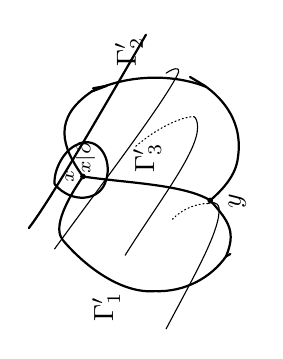
\begin{tikzpicture}[x=.8cm,y=.8cm,line cap=round,line join=round]
\begin{scope}[rotate=90]
\draw[thick] (0,2.02) .. controls (-.48,2.35) and (-.84,2.48) .. (-1.01,2.34)
 .. controls (-1.47,1.95) and (-1.86,1.38) .. (-1.82,.88)
 .. controls (-1.84,.40) and (-1.60,-.02) .. (-1.27,-.25)
 .. controls (-.89,-.41) and (-.72,-.31) .. (-.38,0);
\draw[thick] (0,2.02) .. controls (.47,2.36) and (.92,2.51) .. (1.35,1.88)
 .. controls (1.67,1.19) and (1.59,.47) .. (1.42,.06)
 .. controls (1.14,-.32) and (.75,-.51) .. (.30,-.44)
 .. controls (.03,-.41) and (-.19,-.22) .. (-.38,0);
\draw[thick] (0,2.02) .. controls (-.10,1.38) and (-.12,.42) .. (-.38,0);
\draw[thick] (-.12,2.47) .. controls (.10,2.49) and (.43,2.32) .. (.51,2.10)
 .. controls (.66,1.78) and (.28,1.55) .. (-.05,1.65)
 .. controls (-.41,1.74) and (-.43,2.22) .. (-.12,2.47);
\draw[thick] (1.35,1.88) -- (1.44,1.64) -- (1.40,1.86);
\draw[thick] (1.43,.07) -- (1.58,.32);
\draw[thick] (-1.27,-.25) -- (-1.23,-.32);
\draw[thick] (-.82,2.88) .. controls (-.40,2.55) and (1.18,1.64) .. (2.25,1.02);
\draw (-.82,2.88) -- (-.27,2.50);
\draw (-1.15,2.47) .. controls (-.25,1.82) and (1.25,.67) .. (1.66,.50)
 .. controls (1.75,.48) and (1.71,.60) .. (1.64,.70);
\draw (-1.25,1.35) .. controls (-.42,.83) and (.38,.20) .. (.78,.20)
 .. controls (.88,.20) and (.94,.23) .. (.95,.26);
\draw (-2.42,.70) .. controls (-1.60,.27) and (-.85,-.17) .. (-.50,-.14)
 .. controls (-.39,-.12) and (-.41,-.01) .. (-.43,.04);
\draw[densely dotted] (.48,1.18) .. controls (.79,.82) and (.95,.44) .. (.95,.26);
\draw[densely dotted] (-.68,.60) .. controls (-.50,.43) and (-.43,.20) .. (-.43,.04);
\fill (0,2.02) circle (.045);
\fill (-.38,0) circle (.045);
\node[rotate=90] at (-2.07,1.65) {$\Gamma'_1$};
\node[rotate=90] at (1.98,1.29) {$\Gamma'_2$};
\node[rotate=90] at (.30,1.00) {$\Gamma'_3$};
% The x-like glyph is already marked at its first occurrence in the set above.
\node[rotate=90,inner sep=0pt] at (0,2.23) {\scriptsize $x$};
\node[rotate=90,inner sep=0pt] at (.30,1.98) {\scriptsize $\deleted{\unsure{x|\partial}}$};
\node[rotate=90] at (-.40,-.43) {$y$};
\end{scope}
\end{tikzpicture}}}
\end{minipage}\hfill
\begin{minipage}[c]{.64\linewidth}
\[
\resizebox{\linewidth}{!}{$\displaystyle
\Gamma_3^{\deleted{\circ}}=\Gamma''_1\cup\Gamma''_{\unsure{2|1}}\cup\partial
\ \big|\quad U_3=V_1\cup V_2\cup\Gamma''_3\quad\big|\quad V_3$}
\]

\[
\dot U_3=\Gamma_3\qquad U_3\cup
\]
\end{minipage}

\[
\unsure{\cdot}\ U,C,V
\]
% archive sheet number: 2


\scanpage{4}
\begingroup\ttfamily

% letterhead
\noindent
\begin{minipage}[t]{.48\linewidth}\centering
U N I V E R S I T E\\
DES SCIENCES ET TECHNIQUES\\
DU LANGUEDOC\\
{\footnotesize $\frown\frown\frown\frown\frown\frown\frown\frown\frown\frown\frown\frown$}\\[.6em]
Service de la Scolarité\\
JP/GJ\\[.5em]
\uline{Diffusion} : Liste A\\
N°: 2418
\end{minipage}\hfill
\begin{minipage}[t]{.49\linewidth}\raggedleft
MONTPELLIER, le 19 AVRIL 1977\\
\end{minipage}

\begin{center}
\uline{AVIS DE SOUTENANCE D'UNE THESE DE DOCTORAT DE}\\[.5em]
\uline{SPECIALITE : SCIENCES DE LA TERRE mention GEOLOGIE APPLIQUEE}
\end{center}

\uline{Nom et prénom du candidat} : BAYER Michel

\uline{Titre de la thèse} : Etude gravimétrique de la Corse.

\uline{Date, heure et lieu de soutenance prévus} : 25 AVRIL 1977 à 14 h. 30

\hspace*{3em}Salle de cours n° 10 - U.S.T.L.

\uline{Nom du Directeur de thèse} : M. LOUIS Pierre

\uline{Désignation du laboratoire où la thèse est préparée} :

\hspace*{3em}Laboratoire de Géophysique

\uline{Analyse de l'ouvrage} : Afin de terminer le levé gravimétrique de la Corse, 270 mesures ont été effectuées. L'ensemble des données (720 stations) a été traité (cartes de l'anomalie de Bouguer, dérivées, régionales et résiduelles) puis interprété, en tenant compte de la géologie et de l'aéromagnétisme. Des hypothèses sont proposées, en particulier pour la structure profonde de la Corse et des régions avoisinantes (bassin Algéro-provençal).

\uline{Durée approximative des recherches ayant abouti à la thèse} : Deux ans

\uline{Composition du jury proposé} :

\begin{center}
\begin{tabular}{r@{\quad}l}
MM. : & P. LOUIS\\
      & M. MATTAUER\\
      & R. NEUMANN\\
Mlle  & F. RIMBERT\\
M.    & J. ORSINI
\end{tabular}
\end{center}

\noindent\hfill\begin{minipage}{.49\linewidth}\centering
Le Secrétaire Général,\\[.7em]
\figure{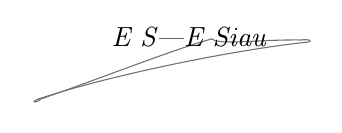
\begin{tikzpicture}[x=.70cm,y=.70cm,line cap=round]
\draw[thin,black!55] (-2.22,-.72) .. controls (-2.32,-.82) and (-2.45,-.77) .. (-2.20,-.70)
 .. controls (-.96,-.29) and (1.27,.17) .. (2.61,.31)
 .. controls (2.72,.33) and (2.66,.37) .. (2.50,.35)
 .. controls (1.70,.36) and (1.04,.25) .. (.88,.37);
% The second long edge rises from the left return into the autograph.
\draw[thin,black!55] (-2.22,-.72)
 .. controls (-1.28,-.40) and (.16,.17) .. (.88,.37);
\node[anchor=base,inner sep=0pt] at (.46,.23) {\normalfont\itshape\handwritten{\unsure{E S|E Siau}}};
\end{tikzpicture}}
\uline{E. SIAU}\\
\end{minipage}
\endgroup
% archive pencil sheet number: 3 (lower-left margin; not a manuscript page number)


\scanpage{6}

$\unsure{\mathcal{X}|\mathscr{X}}$ qui est aussi la somme amalgamée de\deleted{\unsure{s}} $\overline W$ et de\deleted{s} $\coprod_{i\in I}\overline U_i$ (\unsure{sur}
\diagram{\begin{tikzcd}[ampersand replacement=\&,row sep=small,column sep=large]
\coprod_i B_i \arrow[r,hook] \arrow[dr] \& \overline W\\
\& \coprod_i\overline U_i
\end{tikzcd}}
) :

\noindent\begin{minipage}[c]{.41\linewidth}
\figure{\resizebox{\linewidth}{!}{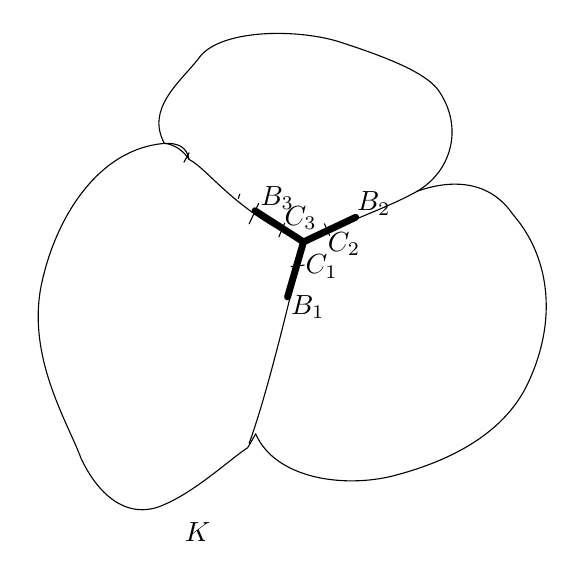
\begin{tikzpicture}[x=.92cm,y=.92cm,line cap=round,line join=round]
\draw (-1.92,1.36) .. controls (-2.18,1.84) and (-1.71,2.20) .. (-1.45,2.53)
 .. controls (-1.18,2.93) and (-.14,2.95) .. (.47,2.77)
 .. controls (1.09,2.57) and (1.65,2.36) .. (1.85,2.11)
 .. controls (2.22,1.60) and (2.05,.98) .. (1.57,.70);
\draw (-1.92,1.36) .. controls (-2.88,1.28) and (-3.46,.25) .. (-3.63,-.65)
 .. controls (-3.80,-1.63) and (-3.25,-2.50) .. (-3.07,-2.99)
 .. controls (-2.81,-3.54) and (-2.39,-3.85) .. (-1.91,-3.62)
 .. controls (-1.47,-3.43) and (-.99,-2.98) .. (-.77,-2.84) -- (-.66,-2.65);
\draw (-.66,-2.65) .. controls (-.38,-3.29) and (.62,-3.41) .. (1.31,-3.21)
 .. controls (2.26,-2.95) and (2.87,-2.50) .. (3.13,-1.88)
 .. controls (3.51,-1.02) and (3.38,-.18) .. (2.89,.38)
 .. controls (2.57,.85) and (2.05,.87) .. (1.57,.70);
\draw (-1.92,1.36) .. controls (-1.78,1.35) and (-1.65,1.25) .. (-1.58,1.14)
 .. controls (-1.30,.99) and (-.96,.44) .. (0,0);
% Narrow return loop at the upper-left outer junction: both edges are visible.
\draw (-1.92,1.36) .. controls (-1.75,1.37) and (-1.61,1.32) .. (-1.58,1.14);
\draw (0,0) .. controls (.67,.31) and (1.20,.49) .. (1.57,.70);
% The descending divider stops short-left of the lower outer cusp.
\draw (0,0) .. controls (-.23,-.96) and (-.51,-2.12) .. (-.75,-2.78);
\draw[line width=2.5pt] (-.67,.43) -- (0,0) -- (.72,.34);
\draw[line width=2.5pt] (0,0) -- (-.22,-.76);
\draw (-1.65,1.10)--(-1.58,1.23) (-.90,.60)--(-.88,.66) (-.75,.25)--(-.62,.53)
 (-.34,.07)--(-.26,.26) (.36,.09)--(.29,.25) (-.17,-.34)--(.01,-.32);
\node at (-.36,.60) {$B_3$}; \node at (-.04,.33) {$C_3$};
\node at (.97,.53) {$B_2$}; \node at (.56,-.03) {$C_2$};
\node at (.25,-.34) {$C_1$}; \node at (.06,-.90) {$B_1$};
\node at (-1.46,-4.00) {$K$};
\end{tikzpicture}}}
\end{minipage}\hfill
\begin{minipage}[c]{.56\linewidth}
\deleted{L'application \unsure{naturelle}}

\[
\deleted{\unsure{\text{de}}\quad\mathcal{X}\longrightarrow X}
\]

\[
\resizebox{\linewidth}{!}{$\displaystyle
\begin{aligned}
\mathcal X&\simeq\overline W\amalg_{\left(\coprod_i B_i\right)}
 \left(\deleted{\unsure{\bigcup}}\coprod_i\overline U_i\right)\\
&\simeq\coprod_{i\,(\unsure{w|W})}X_i
\end{aligned}
\qquad
\begin{array}{c}
X_{\unsure{w|i}}\simeq\mathcal X_i\\
\phantom{X_i\simeq{}}\shortparallel\\[-.5ex]
\phantom{X_i\simeq{}}\operatorname{Im}X_i
\end{array}$}
\]
\end{minipage}
\margin{\tikz[baseline=-.2ex]{\draw (.58,.34) .. controls (.44,.36) and (.15,.12) .. (0,0); \draw (0,0) .. controls (-.08,.09) and (-.13,.06) .. (-.09,0) .. controls (-.05,-.04) and (.01,-.01) .. (0,0) -- (.08,.025);} ouvert de $\mathcal X$}

$\mathcal X\longrightarrow X$ est étale en les pts de $\mathcal X\smallsetminus\coprod_i C_i$, c'est une imm fermée en les pts de $\coprod C_i$

6) Énoncé d'invariance de $\mathcal X$ par rapport au remplacement de $K$ par $K^*\subset K$ ($U_i,U'_i$ par $U_i^*=U_i\cap K^*$, \inserted{$U_i'{}^{\unsure{\wedge|*}}=U'_i\cap K^\wedge$}), pourvu que
% slanted left-margin note, three lines in its own orientation
\margin{vérifier l'énoncé précis\ldots}
\deleted{$\unsure{\dot K'|K'}\subset\bigcup U_i$, et} \inserted{$\dot K^*\subset\bigcup U_i$, et} $\deleted{(K\smallsetminus K')^{-}}\ \forall i$, $C_i\subset\overline{U_i^*}\cap\overline{U_i'{}^*}$ (- il suffit que $\deleted{\unsure{K^*|K'}}$ $\operatorname{int}K'\supset\bigcup C_i$

-- vérifier si dans les div. hypothèses précédentes, il n'y avait pas lieu d'exiger $\bigcup C_i\subset\operatorname{int}K$ i.e. $C_i\cap\dot K=\varnothing\quad\forall i\in I$\ldots
\margin{\tikz{\draw[line width=.3pt] (0,0) .. controls (-.04,.25) and (-.05,.6) .. (0,.9);}}
% vertical pen stroke to the left of the last line
% Detached short pen stroke below-left of his own page numeral.
\margin{\tikz[baseline=-.2ex]{\draw[line width=.3pt] (0,0) -- (.015,-.07);}}
\mspage{5}
% archive sheet number: 5
